% !TEX root = ../notes_unsupervisedlearning.tex
% Chapter 6: Variational Inference and VAEs
%%%%%%%%%%%%%%%%%%%%%%%%%%%%%%%%%%%%%%%%%%%%%%%%%%%%%%%%%%%%%%%%%%%%%%

\chapter{Variational Inference}\index{VAE}\index{Variational Autoencoder}\index{ELBO}
\newthought{Model data as distributions, not points.}

%═══════════════════════════════════════════════════════════════════════
% BLOCK 1: INTRODUCTION
%═══════════════════════════════════════════════════════════════════════

\section{The Why}

\marginnote{Autoencoders compress, but VAEs generate---and quantify uncertainty.}

Standard autoencoders learn a deterministic mapping: input $\to$ latent code $\to$ reconstruction. But the latent space may be irregular, with "holes" where no data maps. How can we:
\begin{itemize}
    \item Generate new samples by sampling from the latent space?
    \item Interpolate smoothly between data points?
    \item Quantify uncertainty in representations?
\end{itemize}

\textbf{Variational Autoencoders (VAEs)} solve this by learning a \textbf{probabilistic} latent space. Instead of encoding to a point, we encode to a \textbf{distribution}.

\subsection{Hands-On Experience}

\begin{marginfigure}
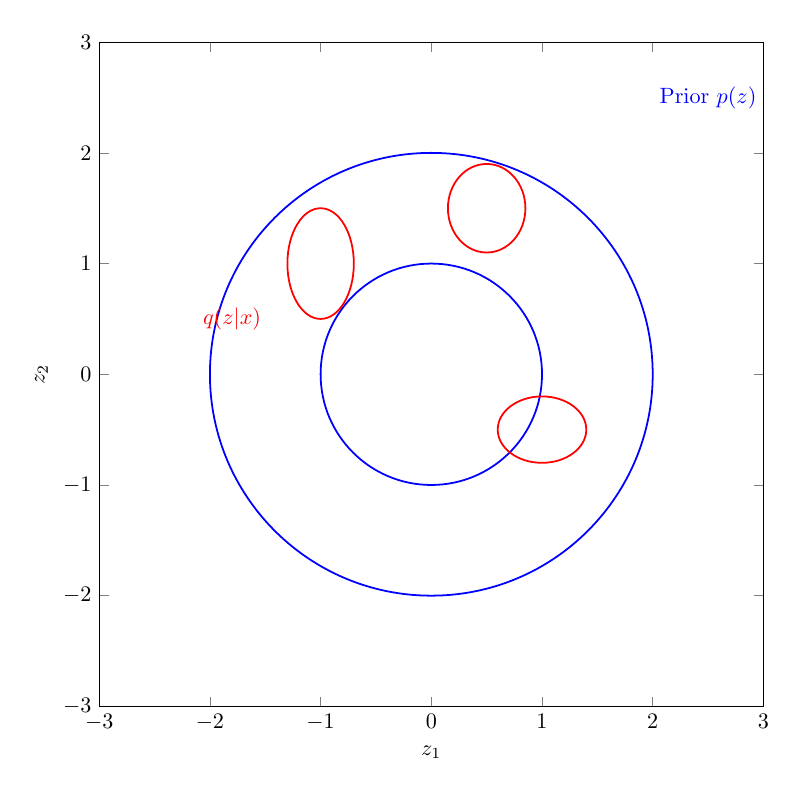
\begin{tikzpicture}[scale=0.8]
    \begin{axis}[
        xlabel={$z_1$},
        ylabel={$z_2$},
        xmin=-3, xmax=3,
        ymin=-3, ymax=3,
        width=\textwidth,
        height=\textwidth,
        axis equal,
    ]
    % Standard normal prior
    \draw[blue, thick] (axis cs:0,0) circle[radius=1];
    \draw[blue, thick] (axis cs:0,0) circle[radius=2];
    % Encoded distributions
    \draw[red, thick] (axis cs:-1,1) ellipse[x radius=0.3, y radius=0.5];
    \draw[red, thick] (axis cs:1,-0.5) ellipse[x radius=0.4, y radius=0.3];
    \draw[red, thick] (axis cs:0.5,1.5) ellipse[x radius=0.35, y radius=0.4];
    % Labels
    \node[blue] at (axis cs:2.5,2.5) {Prior $p(z)$};
    \node[red] at (axis cs:-1.8,0.5) {$q(z|x)$};
    \end{axis}
\end{tikzpicture}
\caption{VAE latent space: each input encodes to a distribution (red ellipses), regularized toward the prior (blue circles).}
\end{marginfigure}

Imagine you have a 2D latent space with a standard normal prior $p(z) = \mathcal{N}(0, I)$.

\begin{enumerate}
    \item Sample $z_1 = (1, 0)$ and $z_2 = (-1, 0)$
    \item Interpolate: $z_t = (1-t) z_1 + t z_2$ for $t \in [0, 1]$
    \item Decode each $z_t$ to get a smooth transition between outputs
\end{enumerate}

This works because VAEs enforce that the latent space is "filled in"---every point can decode to something meaningful.

\subsection{Learning Objectives}

After this lecture, you will be able to:
\begin{enumerate}
    \item Derive the Evidence Lower Bound (ELBO) and explain its components
    \item Implement the reparameterization trick for gradient-based training
    \item Build and train a Variational Autoencoder from scratch
    \item Explore and interpolate in learned latent spaces
    \item Extend to variants: $\beta$-VAE, VQ-VAE, conditional VAE
\end{enumerate}

%═══════════════════════════════════════════════════════════════════════
% BLOCK 2: MAIN THEORY
%═══════════════════════════════════════════════════════════════════════

\section{From Autoencoders to VAEs}

\marginnote{Standard autoencoders: $x \to z \to \hat{x}$, minimize $\|x - \hat{x}\|^2$}

A standard autoencoder has:
\begin{itemize}
    \item \textbf{Encoder}: $f_\phi: x \mapsto z$
    \item \textbf{Decoder}: $g_\theta: z \mapsto \hat{x}$
    \item \textbf{Loss}: $\mathcal{L} = \|x - g_\theta(f_\phi(x))\|^2$
\end{itemize}

\textbf{Problems}:
\begin{enumerate}
    \item Latent space may have "holes"---points $z$ that don't decode to valid data
    \item No principled way to sample new data
    \item No uncertainty quantification
\end{enumerate}

\begin{figure}[h]
\centering
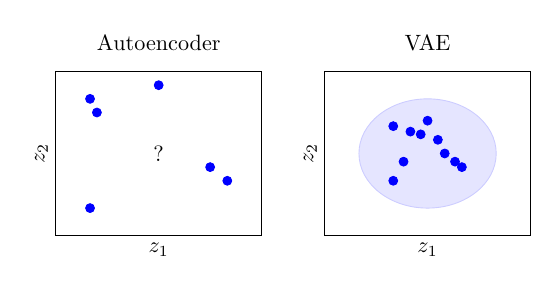
\begin{tikzpicture}[scale=0.8]
    % Autoencoder latent space
    \begin{axis}[
        name=ae,
        title={Autoencoder},
        xlabel={$z_1$}, ylabel={$z_2$},
        xmin=-3, xmax=3, ymin=-3, ymax=3,
        width=0.4\textwidth,
        ticks=none,
    ]
    \addplot[only marks, mark=*, mark size=2pt, blue] coordinates {
        (-2,2) (-1.8,1.5) (2,-1) (1.5,-0.5) (0,2.5) (-2,-2)
    };
    \node at (axis cs:0,0) {?};
    \end{axis}

    % VAE latent space
    \begin{axis}[
        at={(ae.east)}, anchor=west, xshift=1cm,
        title={VAE},
        xlabel={$z_1$}, ylabel={$z_2$},
        xmin=-3, xmax=3, ymin=-3, ymax=3,
        width=0.4\textwidth,
        ticks=none,
    ]
    \draw[blue!20, fill=blue!10] (axis cs:0,0) circle[radius=2];
    \addplot[only marks, mark=*, mark size=2pt, blue] coordinates {
        (-1,1) (-0.5,0.8) (1,-0.5) (0.8,-0.3) (0,1.2) (-1,-1)
        (0.3,0.5) (-0.7,-0.3) (0.5,0) (-0.2,0.7)
    };
    \end{axis}
\end{tikzpicture}
\caption{Autoencoder: sparse, irregular latent space. VAE: regularized, filled latent space.}
\end{figure}


\section{The Evidence Lower Bound (ELBO)}

\marginnote{We want to maximize $\log p(x)$, but this is intractable.}

\subsection{The Problem}

We want to model data with latent variables:
\begin{equation}
    p_\theta(x) = \int p_\theta(x|z) p(z) \, dz
\end{equation}

This integral is intractable for complex decoders. We also want to infer the posterior $p_\theta(z|x)$, which is equally intractable.

\subsection{Variational Inference}

\textbf{Key idea}: Approximate the intractable posterior $p_\theta(z|x)$ with a tractable distribution $q_\phi(z|x)$, parameterized by an encoder network.

\begin{align}
    \log p_\theta(x) &= \log \int p_\theta(x|z) p(z) \, dz \\
    &= \log \int \frac{q_\phi(z|x)}{q_\phi(z|x)} p_\theta(x|z) p(z) \, dz \\
    &= \log \mathbb{E}_{q_\phi(z|x)} \left[ \frac{p_\theta(x|z) p(z)}{q_\phi(z|x)} \right]
\end{align}

By Jensen's inequality ($\log \mathbb{E}[X] \geq \mathbb{E}[\log X]$):

\begin{equation}
    \log p_\theta(x) \geq \mathbb{E}_{q_\phi(z|x)} \left[ \log p_\theta(x|z) + \log p(z) - \log q_\phi(z|x) \right]
\end{equation}

\begin{definition}[Evidence Lower Bound]
\begin{equation}
    \text{ELBO}(\theta, \phi; x) = \underbrace{\mathbb{E}_{q_\phi(z|x)}[\log p_\theta(x|z)]}_{\text{Reconstruction}} - \underbrace{D_{KL}(q_\phi(z|x) \| p(z))}_{\text{Regularization}}
    \label{eq:elbo}
\end{equation}
\end{definition}

\marginnote{ELBO = Evidence Lower BOund. We maximize ELBO to approximately maximize $\log p(x)$.}

\textbf{Interpretation}:
\begin{itemize}
    \item \textbf{Reconstruction term}: Decoder should reconstruct $x$ from sampled $z$
    \item \textbf{KL term}: Encoder distribution should stay close to the prior $p(z) = \mathcal{N}(0, I)$
\end{itemize}


\section{The Reparameterization Trick}

\marginnote{Sampling is not differentiable. The reparameterization trick fixes this.}

To optimize the ELBO, we need gradients through $\mathbb{E}_{q_\phi(z|x)}[\cdot]$. But sampling from $q_\phi(z|x)$ is not differentiable!

\textbf{Solution}: Instead of sampling $z \sim q_\phi(z|x) = \mathcal{N}(\mu_\phi(x), \sigma_\phi^2(x))$, we reparameterize:

\begin{equation}
    z = \mu_\phi(x) + \sigma_\phi(x) \odot \epsilon, \quad \epsilon \sim \mathcal{N}(0, I)
\end{equation}

Now the stochasticity is in $\epsilon$, which doesn't depend on $\phi$. Gradients flow through $\mu$ and $\sigma$.

\begin{figure}[h]
\centering
\begin{tikzpicture}[node distance=1.5cm, auto]
    % Nodes
    \node[draw, rectangle, minimum width=1.5cm] (x) {$x$};
    \node[draw, rectangle, right of=x, xshift=1cm, minimum width=1.5cm] (enc) {Encoder};
    \node[draw, rectangle, above right of=enc, yshift=0.3cm, minimum width=1cm] (mu) {$\mu$};
    \node[draw, rectangle, below right of=enc, yshift=-0.3cm, minimum width=1cm] (sigma) {$\sigma$};
    \node[draw, circle, right of=mu, xshift=1.5cm, yshift=-0.7cm] (times) {$\times$};
    \node[draw, circle, above of=times, yshift=-0.5cm] (plus) {$+$};
    \node[right of=times, xshift=0.5cm] (eps) {$\epsilon \sim \mathcal{N}(0,I)$};
    \node[draw, rectangle, right of=plus, xshift=1.5cm, minimum width=1cm] (z) {$z$};
    \node[draw, rectangle, right of=z, xshift=1cm, minimum width=1.5cm] (dec) {Decoder};
    \node[draw, rectangle, right of=dec, xshift=1cm, minimum width=1.5cm] (xhat) {$\hat{x}$};

    % Arrows
    \draw[->] (x) -- (enc);
    \draw[->] (enc) -- (mu);
    \draw[->] (enc) -- (sigma);
    \draw[->] (mu) -- (plus);
    \draw[->] (sigma) -- (times);
    \draw[->] (eps) -- (times);
    \draw[->] (times) -- (plus);
    \draw[->] (plus) -- (z);
    \draw[->] (z) -- (dec);
    \draw[->] (dec) -- (xhat);
\end{tikzpicture}
\caption{VAE architecture with reparameterization trick: $z = \mu + \sigma \odot \epsilon$.}
\end{figure}


\section{VAE Architecture and Training}

\subsection{Architecture}

\begin{itemize}
    \item \textbf{Encoder} $q_\phi(z|x)$: Neural network outputting $\mu_\phi(x)$ and $\log \sigma^2_\phi(x)$
    \item \textbf{Decoder} $p_\theta(x|z)$: Neural network outputting reconstruction parameters
    \item \textbf{Prior}: $p(z) = \mathcal{N}(0, I)$
\end{itemize}

\subsection{Loss Function}

For Gaussian decoder with fixed variance:
\begin{equation}
    \mathcal{L}(\theta, \phi; x) = \|x - \hat{x}\|^2 + D_{KL}(q_\phi(z|x) \| p(z))
\end{equation}

The KL term has a closed form for Gaussians:
\begin{equation}
    D_{KL}(\mathcal{N}(\mu, \sigma^2) \| \mathcal{N}(0, 1)) = \frac{1}{2} \sum_j \left( \mu_j^2 + \sigma_j^2 - \log \sigma_j^2 - 1 \right)
\end{equation}

\marginnote{In practice, output $\log \sigma^2$ instead of $\sigma$ for numerical stability.}


\section{Exploring the Latent Space}

\subsection{Latent Interpolation}

Given two data points $x_1, x_2$:
\begin{enumerate}
    \item Encode: $z_1 = \mu_\phi(x_1)$, $z_2 = \mu_\phi(x_2)$
    \item Interpolate: $z_t = (1-t) z_1 + t z_2$
    \item Decode: $\hat{x}_t = g_\theta(z_t)$
\end{enumerate}

\subsection{Generation}

Sample $z \sim \mathcal{N}(0, I)$ and decode: $\hat{x} = g_\theta(z)$.


\section{VAE Variants}

\subsection{$\beta$-VAE: Disentanglement}

\marginnote{$\beta$-VAE trades reconstruction quality for disentanglement.}

Increase the weight on the KL term:
\begin{equation}
    \mathcal{L}_\beta = \text{Reconstruction} + \beta \cdot D_{KL}
\end{equation}

With $\beta > 1$, the model is pressured to use the latent space efficiently, often leading to \textbf{disentangled} representations where each dimension corresponds to a single factor of variation.

\subsection{VQ-VAE: Discrete Latents}

\marginnote{VQ-VAE uses discrete codes, enabling powerful autoregressive priors.}

\textbf{Vector Quantized VAE} replaces continuous latents with discrete codes from a learned codebook:
\begin{equation}
    z_q = \arg\min_{e_k \in \text{codebook}} \|z_e - e_k\|
\end{equation}

Benefits: Can learn powerful autoregressive priors (like PixelCNN) over discrete codes.

\subsection{Conditional VAE}

Add conditioning variable $c$ (e.g., class label):
\begin{itemize}
    \item Encoder: $q_\phi(z|x, c)$
    \item Decoder: $p_\theta(x|z, c)$
\end{itemize}

Enables controlled generation: sample $z$, specify $c$, decode.


\section{Brief: Knowledge Distillation}

\marginnote{Distillation: transfer knowledge from a large "teacher" to a small "student".}

\textbf{Knowledge distillation} compresses large models into smaller ones:
\begin{enumerate}
    \item Train a large \textbf{teacher} model
    \item Train a small \textbf{student} to match teacher's outputs
\end{enumerate}

\textbf{Soft labels}: Instead of hard labels, use teacher's softmax outputs:
\begin{equation}
    p_i^{(T)} = \frac{\exp(z_i / T)}{\sum_j \exp(z_j / T)}
\end{equation}
where $T$ is temperature. Higher $T$ $\to$ softer distribution $\to$ more information.

This connects to VAEs: both involve learning compressed representations that preserve essential information.


%═══════════════════════════════════════════════════════════════════════
% BLOCK 3: STUDENT ACTIVATION
%═══════════════════════════════════════════════════════════════════════

\section{Examples \& Exercises}

\subsection{Exercise 1: ELBO Derivation}

Starting from $\log p(x) = \log \int p(x,z) dz$, derive the ELBO by:
\begin{enumerate}
    \item Introducing $q(z|x)$ via importance sampling
    \item Applying Jensen's inequality
    \item Simplifying to reconstruction + KL form
\end{enumerate}

\subsection{Exercise 2: KL Divergence Computation}

Compute $D_{KL}(\mathcal{N}(\mu, \sigma^2) \| \mathcal{N}(0, 1))$ for:
\begin{enumerate}
    \item $\mu = 0, \sigma = 1$ (should be 0)
    \item $\mu = 1, \sigma = 1$
    \item $\mu = 0, \sigma = 2$
\end{enumerate}

\textbf{Solution}:
Using $D_{KL} = \frac{1}{2}(\mu^2 + \sigma^2 - \log \sigma^2 - 1)$:
\begin{enumerate}
    \item $\frac{1}{2}(0 + 1 - 0 - 1) = 0$ ✓
    \item $\frac{1}{2}(1 + 1 - 0 - 1) = 0.5$
    \item $\frac{1}{2}(0 + 4 - \log 4 - 1) = \frac{1}{2}(3 - 1.39) \approx 0.81$
\end{enumerate}

\subsection{Exercise 3: Reparameterization}

Why can't we directly backpropagate through $z \sim \mathcal{N}(\mu, \sigma^2)$?

\textbf{Solution}: Sampling is a stochastic operation without a gradient. The reparameterization $z = \mu + \sigma \epsilon$ moves the stochasticity to $\epsilon$, which is independent of the parameters. Now $\partial z / \partial \mu = 1$ and $\partial z / \partial \sigma = \epsilon$.


\section{Self-Reflection \& Recap}

\subsection{Reflection Questions}
\begin{enumerate}
    \item Why does the KL term encourage a structured latent space?
    \begin{quote}
        \textit{It penalizes deviation from the prior $\mathcal{N}(0,I)$, forcing encodings to overlap and fill the space rather than clustering in isolated regions.}
    \end{quote}

    \item What happens if you set $\beta$ too high in $\beta$-VAE?
    \begin{quote}
        \textit{Reconstructions become poor because the model is forced to use a very compressed latent space. At the extreme, all inputs map to the same distribution (posterior collapse).}
    \end{quote}

    \item How does VQ-VAE differ from standard VAE?
    \begin{quote}
        \textit{VQ-VAE uses discrete latent codes from a learned codebook instead of continuous Gaussians. This enables powerful autoregressive priors and avoids posterior collapse.}
    \end{quote}
\end{enumerate}

\subsection{Key Concepts}
\begin{itemize}
    \item VAEs learn \textbf{probabilistic} latent representations
    \item \textbf{ELBO} = Reconstruction - KL divergence
    \item \textbf{Reparameterization trick} enables end-to-end training
    \item Variants ($\beta$-VAE, VQ-VAE) offer different trade-offs
    \item \textbf{Distillation} compresses models by training on soft labels
\end{itemize}

\subsection{Next Chapter Teaser}
\marginnote{Teaser: From distributions to deviations}
\newthought{We can now model the data distribution.} But what about data points that don't fit? Anomalies, outliers, and out-of-distribution samples reveal the boundaries of our learned structure. The next chapter explores how to detect and evaluate these deviations---crucial for safe deployment of ML systems.
